\documentclass[]{auvsi_doc}
\setkeys{auvsi_doc.cls}{
	AUVSITitle={UAS Requirements Matrix},
	AUVSIRevision=0.0,
	AUVSIDescription={Initial Draft},
	AUVSIAuthor={Kameron Eves},
	AUVSIChecker={John Akagi},
	AUVSILogoPath={./figs/logo.pdf},
	AUVSIDocID={DJ-005}
}

% include extra packages, if needed
\usepackage{rotating}

% Remove Heading Numbers
\setcounter{secnumdepth}{0}

\begin{document}

\begin{AUVSITitlePage}
\begin{artifacttable} 
%\entry{PC-444, 1.0, 10-02-2018, Opportunity development initial stage, Andrew Torgesen, Kameron Eves\, Ryan Anderson\, Jacob Willis\, Tyler Critchfield\, John Akagi}
\entry{RM-001, 0.1, 09-07-2018, Fall camp draft, Brady Moon, Jacob Willis}
\entry{RM-001, 0.2, 09-14-2018, Revisions after design review, Derek Knowles, Kameron Eves}
\entry{RM-001, 1.0, 10-08-2018, Expansion for stage approval, Kameron Eves, Brandon McBride}
\entry{RM-001, 1.1, 10-08-2018, Reordered requirements to match priority, Jacob Willis, Brady Moon}
\entry{RM-001, 1.2, 10-17-2018, Fixed inconsistency in autonomous flight requirement, Andrew Torgesen, Kameron Eves}
\end{artifacttable}
\end{AUVSITitlePage}

%\AUVSIFigure{figs/requirements_matrix.pdf}{0.8\textwidth}{Top-level requirements matrix for the unmanned aerial system.}{fig:reqMat}
%\begin{sidewaysfigure}
	\begin{center}
	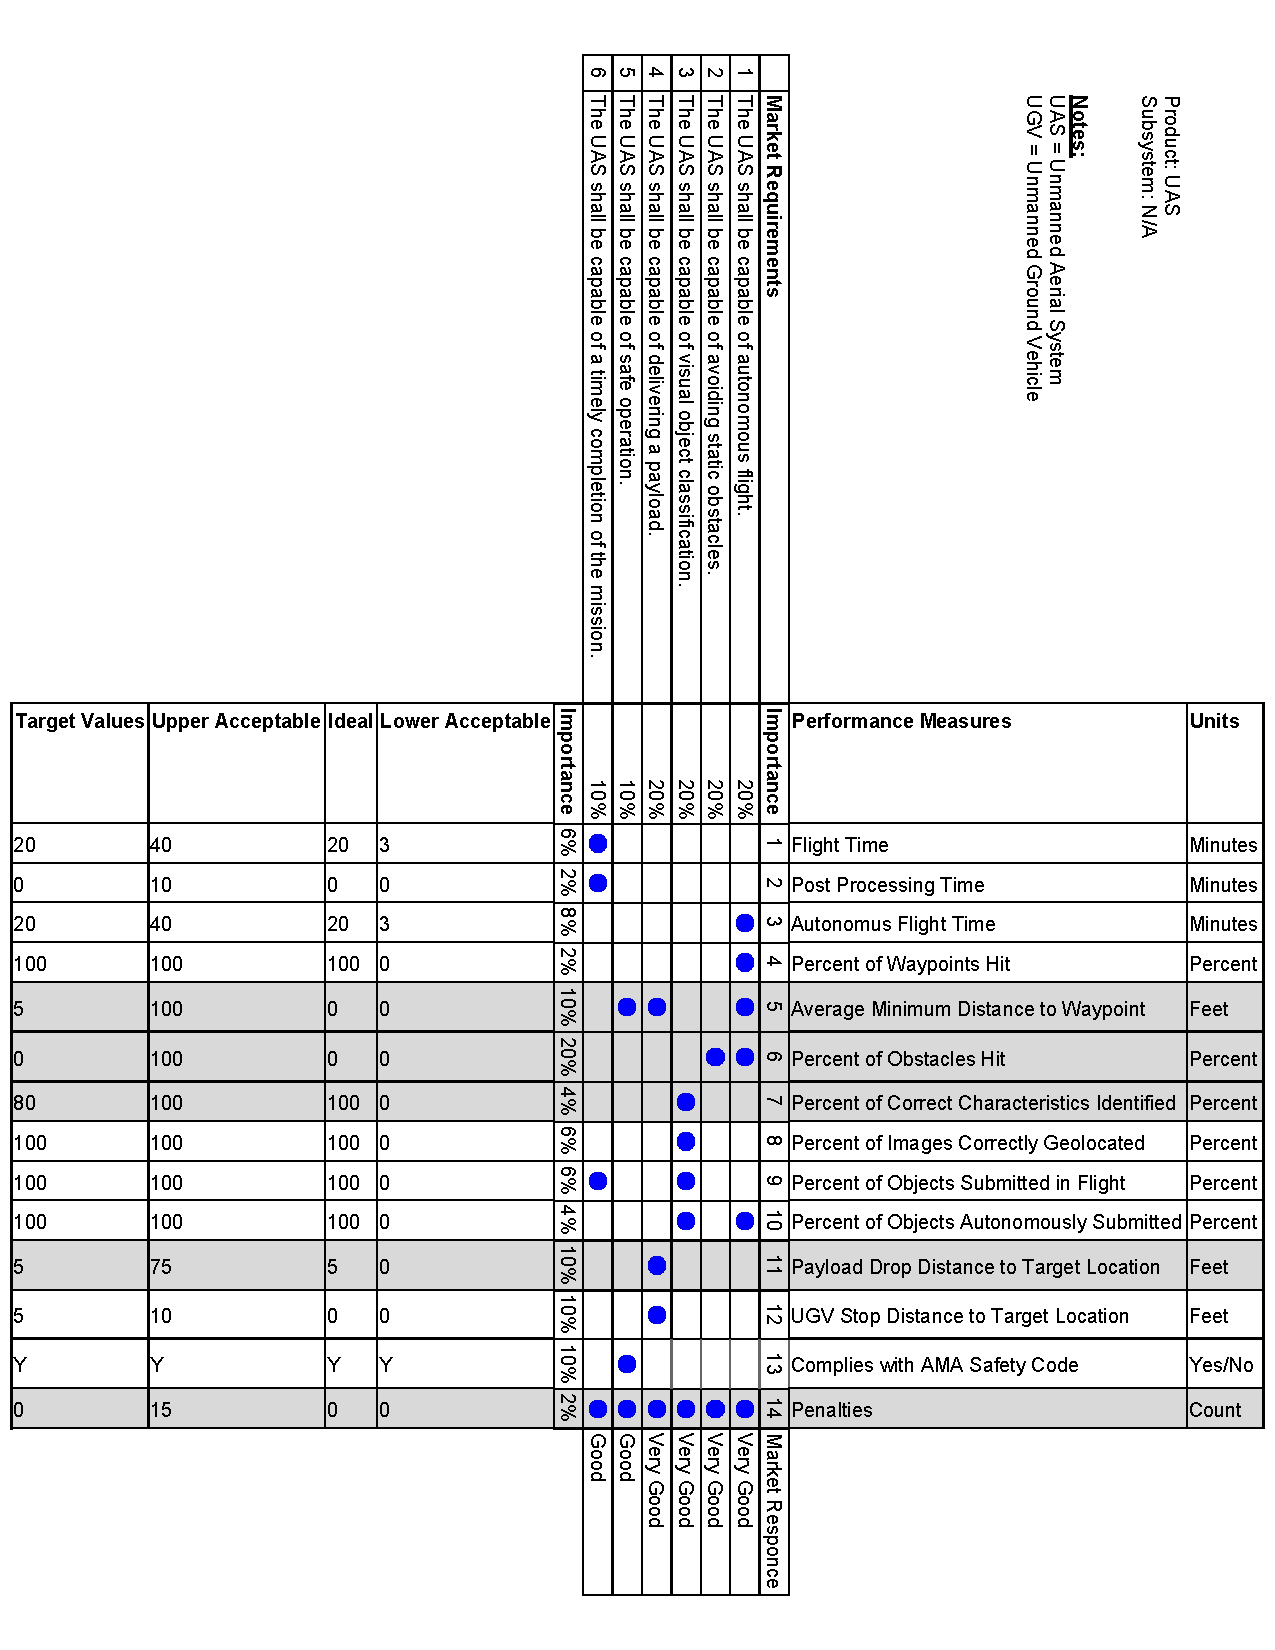
\includegraphics[width=0.8\textwidth]{figs/RequirementsMatrix.pdf}
	\captionof{figure}{Top-level requirements matrix for the unmanned aerial system.}
	\label{fig:reqMat}
	\end{center}
%\end{sidewaysfigure}

\end{document}
